%; whizzy paragraph -pdf xpdf -latex ./whizzypdfptex.sh
%; whizzy-paragraph "^\\\\begin{frame}\\|\\\\emtext"
% latex beamer presentation.
% platex, latex-beamer でコンパイルすることを想定。 

%     Tokyo Debian Meeting resources
%     Copyright (C) 2012 Junichi Uekawa

%     This program is free software; you can redistribute it and/or modify
%     it under the terms of the GNU General Public License as published by
%     the Free Software Foundation; either version 2 of the License, or
%     (at your option) any later version.

%     This program is distributed in the hope that it will be useful,
%     but WITHOUT ANY WARRANTY; without even the implied warreanty of
%     MERCHANTABILITY or FITNESS FOR A PARTICULAR PURPOSE.  See the
%     GNU General Public License for more details.

%     You should have received a copy of the GNU General Public License
%     along with this program; if not, write to the Free Software
%     Foundation, Inc., 51 Franklin St, Fifth Floor, Boston, MA  02110-1301 USA

\documentclass[cjk,dvipdfmx,12pt]{beamer}
\usetheme{Tokyo}
\usepackage{monthlypresentation}

%  preview (shell-command (concat "evince " (replace-regexp-in-string "tex$" "pdf"(buffer-file-name)) "&")) 
%  presentation (shell-command (concat "xpdf -fullscreen " (replace-regexp-in-string "tex$" "pdf"(buffer-file-name)) "&"))
%  presentation (shell-command (concat "evince " (replace-regexp-in-string "tex$" "pdf"(buffer-file-name)) "&"))

%http://www.naney.org/diki/dk/hyperref.html
%日本語EUC系環境の時
\AtBeginDvi{\special{pdf:tounicode EUC-UCS2}}
%シフトJIS系環境の時
%\AtBeginDvi{\special{pdf:tounicode 90ms-RKSJ-UCS2}}

\newenvironment{commandlinesmall}%
{\VerbatimEnvironment
  \begin{Sbox}\begin{minipage}{1.0\hsize}\begin{fontsize}{8}{8} \begin{BVerbatim}}%
{\end{BVerbatim}\end{fontsize}\end{minipage}\end{Sbox}
  \setlength{\fboxsep}{8pt}
% start on a new paragraph

\vspace{6pt}% skip before
\fcolorbox{dancerdarkblue}{dancerlightblue}{\TheSbox}

\vspace{6pt}% skip after
}
%end of commandlinesmall

\title{Debian と systemd}
\subtitle{東京エリアDebian勉強会/OSC 2015 Tokyo Fall\\第132回 2015年10月度 2回目}
\author{岩松 信洋}
\date{2015年10月24日}
\logo{
\includegraphics[width=8cm]{image200607/openlogo-light.eps}}

\begin{document}

\begin{frame}
\titlepage{}
\end{frame}

\begin{frame}{自己紹介}
\begin{itemize}
  \item ソフトウェアエンジニア
  \item Debian Project Official Developer
  \item Bluez, Mozc, Erlang 周りのパッケージメンテナ
  \item 2015年度 Debian JP Project Leader
  \item Linux kernel 開発、U-Boot Custodian、XFCE 日本語コーディネータ、Yocto Project 開発
 \end{itemize}
\end{frame}

\begin{frame}{Agenda}
  \begin{itemize}
   \item systemd とは
   \item systemd への移行と起きた事柄
   \item systemd を使用せずに Debian を利用するには
   \item 今後のイベント
  \end{itemize}
\end{frame}

\section{systemd とは}
\emtext{systemd とは}

\begin{frame}{systemd}
\begin{itemize}
\item init プログラムの一つ

      init とは カーネルが呼ぶ最初のプログラムの総称

      \end{itemize}
\end{frame}

\begin{frame}{systemd}

\begin{minipage}{0.55\hsize}
ブートシーケンス
\begin{enumerate}
\item 電源投入 $\rightarrow$ BIOS または UEFI が起動
\item BIOS または UEFI $\rightarrow$  ブートローダを起動
\item ブートローダ $\rightarrow$ カーネル を起動
\item カーネル $\rightarrow$ init を起動
\end{enumerate}
\end{minipage}
\begin{minipage}{0.39\hsize}
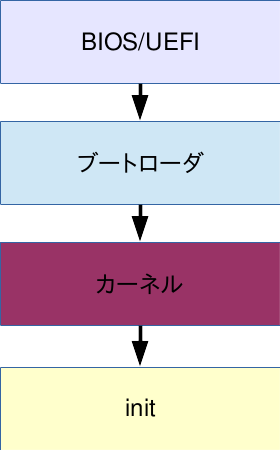
\includegraphics[width=0.8\hsize]{image201510/boot_seq.png}
\end{minipage}

\end{frame}

\begin{frame}{systemd}
\begin{itemize}
\item init プログラムの一つ

      init とは カーネルが呼ぶ最初のプログラムの総称

\item cgroup によるプロセス管理
\item デーモンの並列処理
\item shell を使わない設定
\item linux 専用 init プログラム
\item Debian、Ubuntu、RedHat などの主要 Linux ディストリビューションのデフォルトinit プログラムとして採用されている。
\end{itemize}
\end{frame}

\section{systemd への移行とDebian 界隈で起きた事柄}
\emtext{systemd への移行とDebian 界隈で起きた事柄}

\begin{frame}{2014年2月11日}

\begin{itemize}
\item Debian 8.0 からデフォルト init システム が sysvinit から systemd に。
\item Debian 技術委員会(Debian Technical Committee: Debian プロジェクト内の技術的な論争について最終判断を下す委員会)が決定したもの。

\url{https://lists.debian.org/debian-ctte/2014/02/msg00402.html}

\url{https://bugs.debian.org/727708}

\end{itemize}

\end{frame}



\begin{frame}{2014年9月19日}

\begin{itemize}
\item デフォルトの init システム が systemd になり、インストーラのデフォルト デスクトップ環境に関しても再考される。
\item その結果、Xfce から GNOME3 に変更される。
      \url{https://anonscm.debian.org/cgit/tasksel/tasksel.git/commit/?id=dce99f5f8d84e4c885e6beb4cc1bb5bb1d9ee6d7}
      \footnote{init システム が systemd でなくても GNOME3は動作する。}

\end{itemize}

\end{frame}

\begin{frame}{2014年10月16日}

\begin{itemize}
\item Ian Jackson が init システムの選択の自由を残しておくべきでは、と
systemdを使用しないシステムのサポートをパッケージメンテナに求める一般決議を提案。
\item 支持者が集まり、一般決議が行われることになったが、結果不成立。

\url{https://lists.debian.org/debian-vote/2014/10/msg00001.html}

\item Jessie フリーズ直前での提案に不満が出る。
\item 技術決定プロセスの問題が露呈される。

\end{itemize}

\end{frame}

\begin{frame}{その結果…}


\begin{itemize}
\item Joey Hess が Debian Developer を辞める

debconf、debhelper、alian、ikiwiki などの開発者

\item Colin Watson、Russ Allbery、Ian Jackson が Debian 技術委員会 を辞める
\item Tollef Fog Heen が systemd メンテナから辞める

その後 Debian 技術委員会 メンバに。

\end{itemize}

\end{frame}

\begin{frame}{2014年11月28日}

そして Devuanプロジェクトが立ち上がる。

\begin{center}

\includegraphics[width=1\hsize]{image201510/Devuan-logo.png}
\end{center}

\begin{itemize}
\item Debian ベースの systemd を使わないOSを提供するプロジェクト
\item i386, amd64, armhf のイメージとインストーラを頒布
\item udev の代替プログラムであるvdevを開発
\item \url{http://files.devuan.org/}
\end{itemize}

\end{frame}

\begin{frame}[containsverbatim]

\begin{itemize}

\item 2015/4/21 Ubuntu 15.04 リリース

    init システムに systemd を採用したはじめてのリリース

\item 2015/4/25 Debian 8.0 (コードネーム Jessie)リリース

\end{itemize}

\end{frame}

\begin{frame}
\begin{itemize}
\item 優秀な開発者がプロジェクトなどから抜ける
\item Devuan プロジェクトが立ち上がる
\item それでも Debian 8.0 は予定通りリリースされた
\end{itemize}
\end{frame}

\section{systemd を使用せずに Debian を利用するには}
\emtext{systemd を使用せずに Debian を利用するには}

\begin{frame}[containsverbatim]
Debian では systemd になってもデーモンに対する操作方法は変わらない

\begin{itemize}
\item 例: apache2 start
\begin{commandline}
$ sudo service apache2 start
\end{commandline}

\item 例: apache2 stop
\begin{commandline}
$ sudo service apache2 stop
\end{commandline}

\end{itemize}

\end{frame}

\begin{frame}[containsverbatim]{sysvinit への切り替え}

Debian の init システムを sysvinit に切り替えたい。

\begin{itemize}
\item systemd 嫌い
\item sysvinit のほうに慣れている
\item 独自サービスメンテナンスのため
\end{itemize}

\end{frame}

\begin{frame}[containsverbatim]{sysvinitへの切り替え}

\begin{commandline}
$ sudo apt-get install sysvinit-core
\end{commandline}

\end{frame}


\begin{frame}{sysvinitへの切り替え}

変更点
\begin{itemize}
\item init が systemd から sysvinit に
\item systemd-sysv パッケージが削除され、/sbin/init のシンボリックリンクがなくなる
\item 変わりに sysvinit の /sbin/init バイナリがインストールされる
\item init による cgroups のコントロールがなくなる
\item systemd に依存しているソフトウェアが動作しなくなる\\
	GDM、lightdm など
\end{itemize}

\end{frame}

\begin{frame}[containsverbatim]{sysvinitへの切り替え}

systemd に依存しているソフトウェアの救済

\begin{itemize}
\item systemd-shim パッケージ
\begin{commandline}
$ sudo apt-get install systemd-shim
\end{commandline}
\item systemd からパッケージとして分離できない機能を提供
\item cgroup は cgmanager で管理。cgm コマンドを使って処理

\end{itemize}

\end{frame}

\begin{frame}{sysvinitへの切り替え}
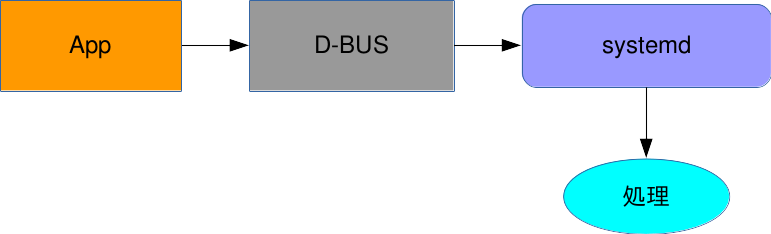
\includegraphics[width=1\hsize]{image201510/shim0.png}
\end{frame}

\begin{frame}{sysvinitへの切り替え}
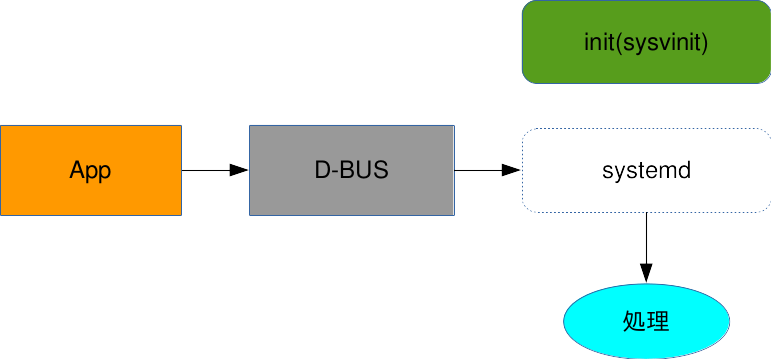
\includegraphics[width=1\hsize]{image201510/shim1.png}
\end{frame}

\begin{frame}{sysvinitへの切り替え}
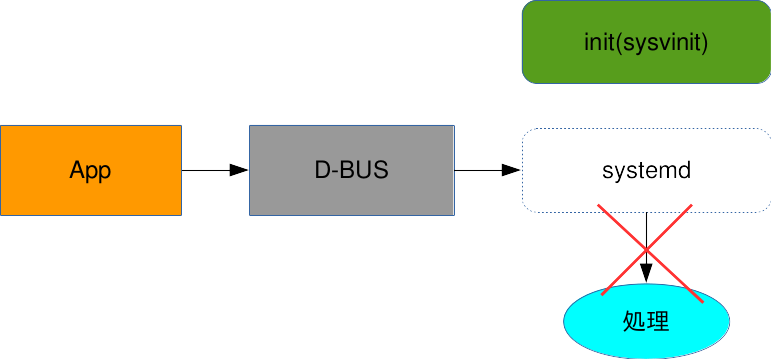
\includegraphics[width=1\hsize]{image201510/shim2.png}
\end{frame}

\begin{frame}{sysvinitへの切り替え}
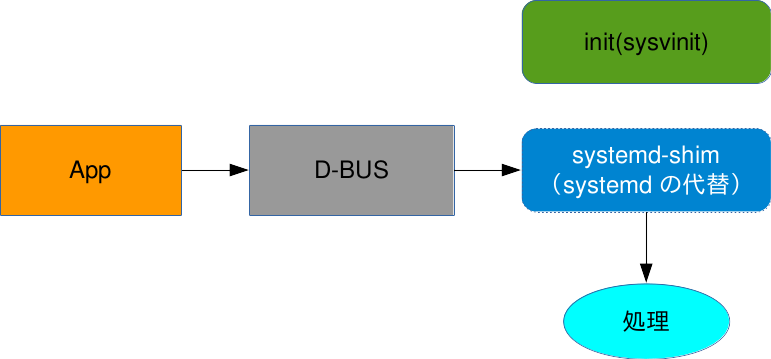
\includegraphics[width=1\hsize]{image201510/shim3.png}
\end{frame}

%\begin{frame}[containsverbatim]
%
%systemd の場合はshutdown は以下のように実行されるが、
%\begin{commandline}
%$ gdbus call -y -d org.freedesktop.systemd1 \
%	-o /org/freedesktop/systemd1 \
%    	-m org.freedesktop.systemd1.Manager.StartUnit \
%	'shutdown.target' ''
%\end{commandline}
%
%\item cgroup は cgmanager で管理。cgm コマンドを使って処理。
%\end{itemize}
%
%\end{frame}

\begin{frame}[containsverbatim]{sysvinit スクリプト}

\begin{itemize}
\item systemd になったら /etc/init.d 以下はどうなるのか
\item /lib/lsb/init-functions によるラッパーがある
\item apache2 を例にして説明

\end{itemize}

\end{frame}


%
%\begin{commandline}
%67 if [ -f /etc/default/rcS ]; then
%68         . /etc/default/rcS
%69 fi
%70 . /lib/lsb/init-functions
%71 
%72 
%73 # Now, set defaults:
%74 APACHE2CTL="$ENV apache2ctl"
%\end{commandline}
%
%\end{frame}
%
%\begin{frame}[containsverbatim]
%
%\texttt{/lib/lsb/init-functions}
%
%\begin{commandline}
%425 log_action_end_msg_post () { :; }
%426 
%427 # Include hooks from other packages in /lib/lsb/init-functions.d
%428 for hook in $(run-parts --lsbsysinit --list /lib/lsb/init-functions.d
%2>/dev/null); do
%429     [ -r $hook ] && . $hook || true
%430 done
%431 
%432 FANCYTTY=
%\end{commandline}
%
%\end{frame}
%
%
%
%\begin{frame}[containsverbatim]
%
%\texttt{/lib/lsb/init-functions.d/40-systemd}
%
%\begin{commandline}
%_use_systemctl=0
%if [ -d /run/systemd/system ]; then
%
%    if [ -n "${DPKG_MAINTSCRIPT_PACKAGE:-}" ]; then
%    # If we are called by a maintainer script, chances are good that a
%    # new or updated sysv init script was installed.  Reload daemon to
%    # pick up any changes.
%        systemctl daemon-reload || true
%    fi
%
%    # Redirect SysV init scripts when executed by the user
%    if [ $PPID -ne 1 ] && [ -z "${init:-}" ] && [ -z
%"${_SYSTEMCTL_SKIP_REDIRECT:-}" ]; then
%        case $(readlink -f "$0") in
%            /etc/init.d/*)
%                _use_systemctl=1
% 
%
%(中略)
%
%systemctl_redirect () {
%    local s
%    local rc
%    local prog=${1##*/}
%    local command=$2
%
%    case "$command" in
%        start)
%            s="Starting $prog (via systemctl)"
%            ;;
%        stop)
%            s="Stopping $prog (via systemctl)"
%            ;;
%        reload|force-reload)
%            s="Reloading $prog configuration (via systemctl)"
%            ;;
%        restart)
%            s="Restarting $prog (via systemctl)"
%            ;;
%    esac
%
%    service="${prog%.sh}.service"
%
%(中略)
%
%    [ "$command" = status ] || log_daemon_msg "$s" "$service"
%    /bin/systemctl $sctl_args $command "$service"
%    rc=$?
%    [ "$command" = status ] || log_end_msg $rc
%
%    return $rc
%}
%
%if [ "$_use_systemctl" = "1" ]; then
%    # Some init scripts use "set -e" and "set -u", we don't want that
%    # here
%    set +e
%    set +u
%
%    if  [ "x$1" = xstart -o \
%        "x$1" = xstop -o \
%        "x$1" = xrestart -o \
%        "x$1" = xreload -o \
%        "x$1" = xforce-reload -o \
%        "x$1" = xstatus ] ; then
%
%        systemctl_redirect $0 $1
%        exit $?
%    fi
%fi
%\end{commandline}
%
%\end{frame}
%
%
%\begin{frame}[containsverbatim]
%
%\begin{commandline}
%$ sudo /etc/init.d/networking restart
%[....] Restarting networking (via systemctl): networking.serviceWarning: networking.service changed on disk. Run
%'systemctl daemon-reload' to reload units.
%. ok 
%
%\end{commandline}
%
%\end{frame}
%
%\begin{frame}
%	systemd 対応デーモン
%	対応率
%
%	sysvinit と systemd の対応方法について
%
\begin{frame}
\begin{center}
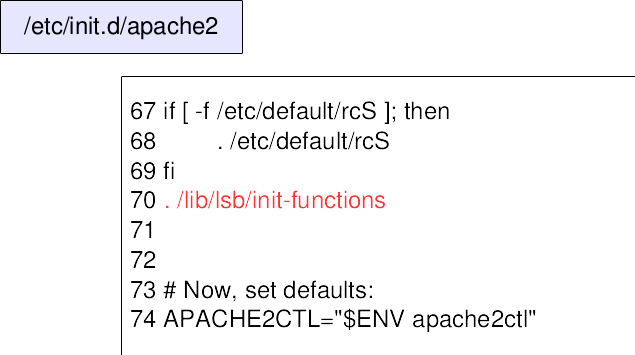
\includegraphics[width=0.8\hsize]{image201510/daemonscript0.png}
\end{center}
\end{frame}

\begin{frame}
\begin{center}
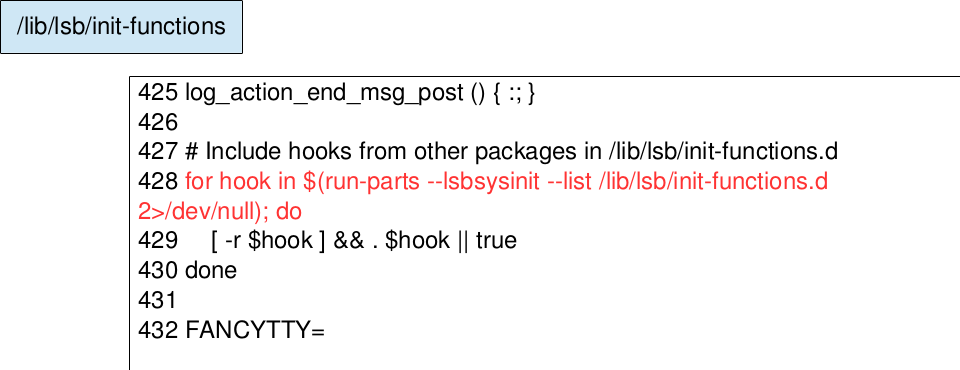
\includegraphics[width=1\hsize]{image201510/daemonscript1.png}
\end{center}
\end{frame}

\begin{frame}
\begin{center}
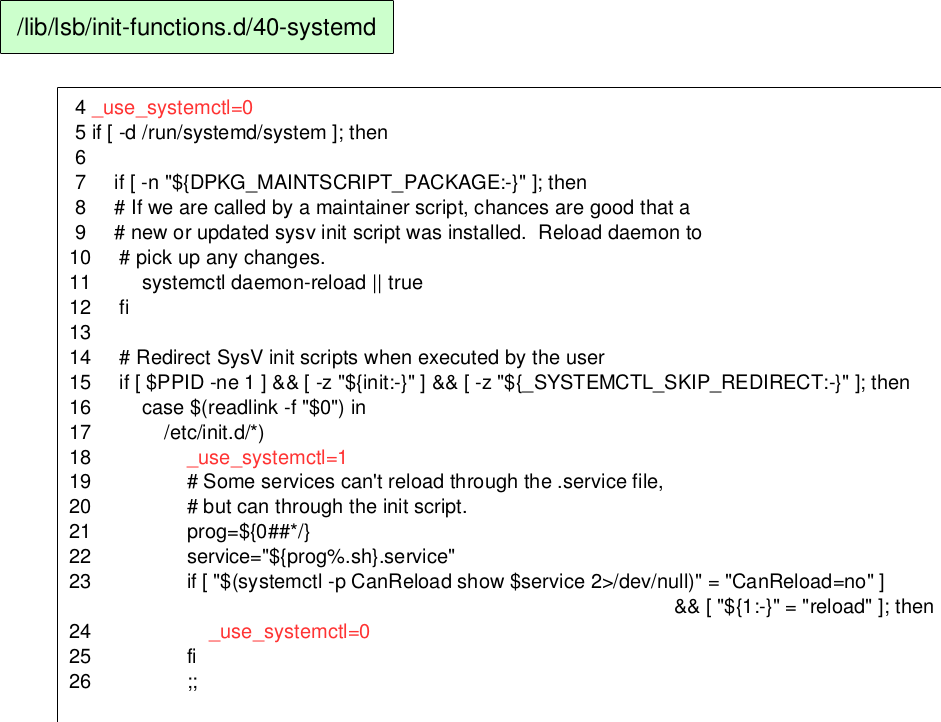
\includegraphics[width=1\hsize]{image201510/daemonscript2.png}
\end{center}
\end{frame}

\begin{frame}
\begin{center}
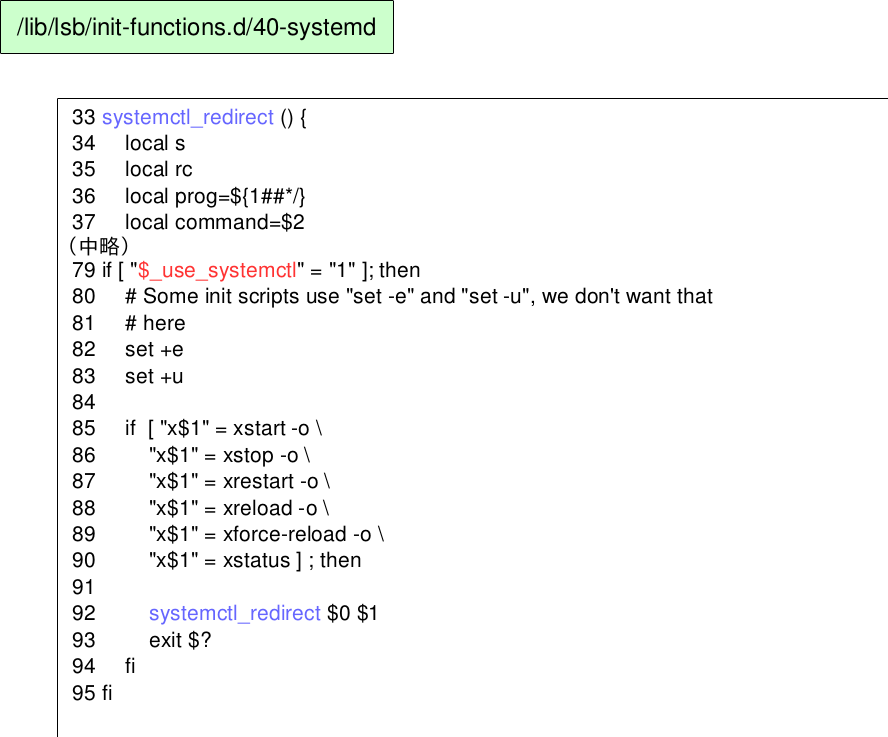
\includegraphics[width=1\hsize]{image201510/daemonscript3.png}
\end{center}
\end{frame}

\begin{frame}
\begin{center}
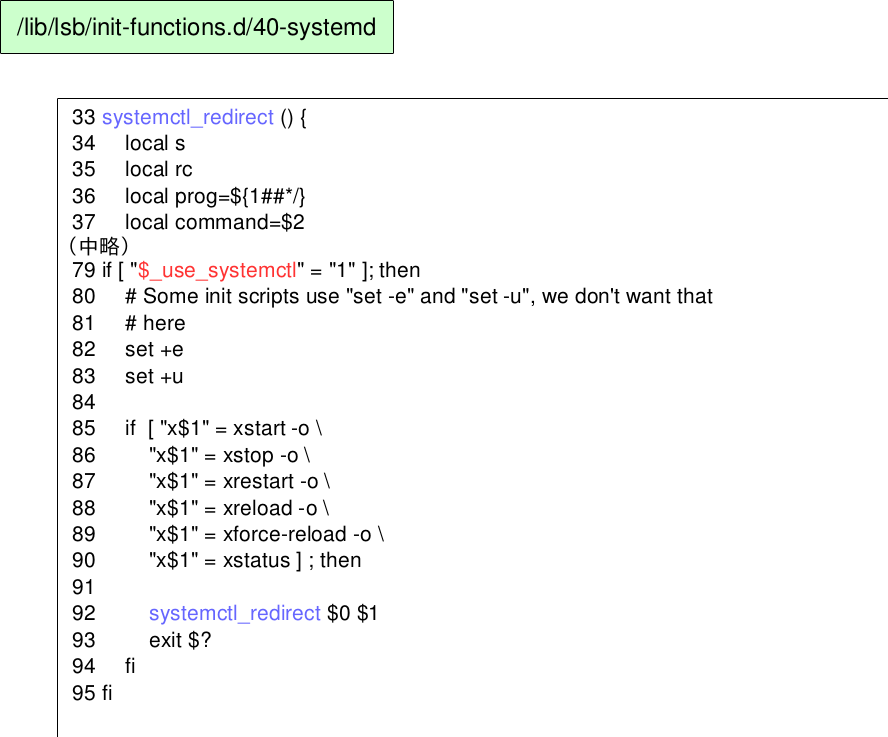
\includegraphics[width=1\hsize]{image201510/daemonscript3.png}
\end{center}
\end{frame}

\begin{frame}
\begin{itemize}
\item /lib/lsb/init-functions を使ってないデーモンがあるのでは?
\item lintian の \texttt{init.d-script-does-not-source-init-functions} に引っかかっているものは要注意

\url{https://lintian.debian.org/tags/init.d-script-does-not-source-init-functions.html}
\end{itemize}
\end{frame}

\begin{frame}{まとめ}

\begin{itemize}
\item Debian では systemd を使わないで運用できる
\item systemd を削除した場合はsystemd-shim をインストールしておくとよい
\item サービス関連はいままでのコマンドがそのまま使える
\item /etc/init.d/ 以下は systemd と sysvinit でも両方使えるようになっている
\end{itemize}

\end{frame}

\section{質問}
\emtext{質問}
\begin{frame}{質問}
何か質問はありますか?
\end{frame}

\section{ブース}
\emtext{ブース}
\begin{frame}{ブース出しています}
ブース出しています。よかったら寄ってください!
\end{frame}

\section{今後のイベント}
\emtext{今後のイベント}
\begin{frame}{今後のイベント}
\begin{itemize}
\item 2015/11/7 (土) KOF 2015 出展\&発表。\\
\url{https://k-of.jp/2015/}
\item 2015/11/21(土) 14:00-19:00 第133回東京エリアDebian勉強会
\end{itemize}
\end{frame}


\end{document}

;;; Local Variables: ***
;;; outline-regexp: "\\([ 	]*\\\\\\(documentstyle\\|documentclass\\|emtext\\|section\\|begin{frame}\\)\\*?[ 	]*[[{]\\|[]+\\)" ***
;;; End: ***
